\section{Проектирование базы знаний интеллектуальной системы}
\label{sec:designing}

\subsection{Общая архитектура интеллектуальной системы и место базы знаний}

% Требования:
% - описать состав основных подсистем: база знаний, решатель задач, интерфейс, внешние сервисы и т.п.;
% - показать место базы знаний в общей архитектуре и основные связи (какие компоненты обращаются к БЗ, кто её модифицирует);
% - привести архитектурную схему верхнего уровня.

Интеллектуальная система «TechInterview» построена по модульно-компонентному принципу, где база знаний фундаментальных основ Computer Science выступает центральным семантическим ядром для хранения, структурирования и выдачи материалов. Декомпозиция на четыре предметные области уровня 1 и интеграционный уровень 0 обеспечивает масштабируемость и кросс-доменную навигацию \cite{Martin2017}. 

\begin{figure}[h]
    \centering
    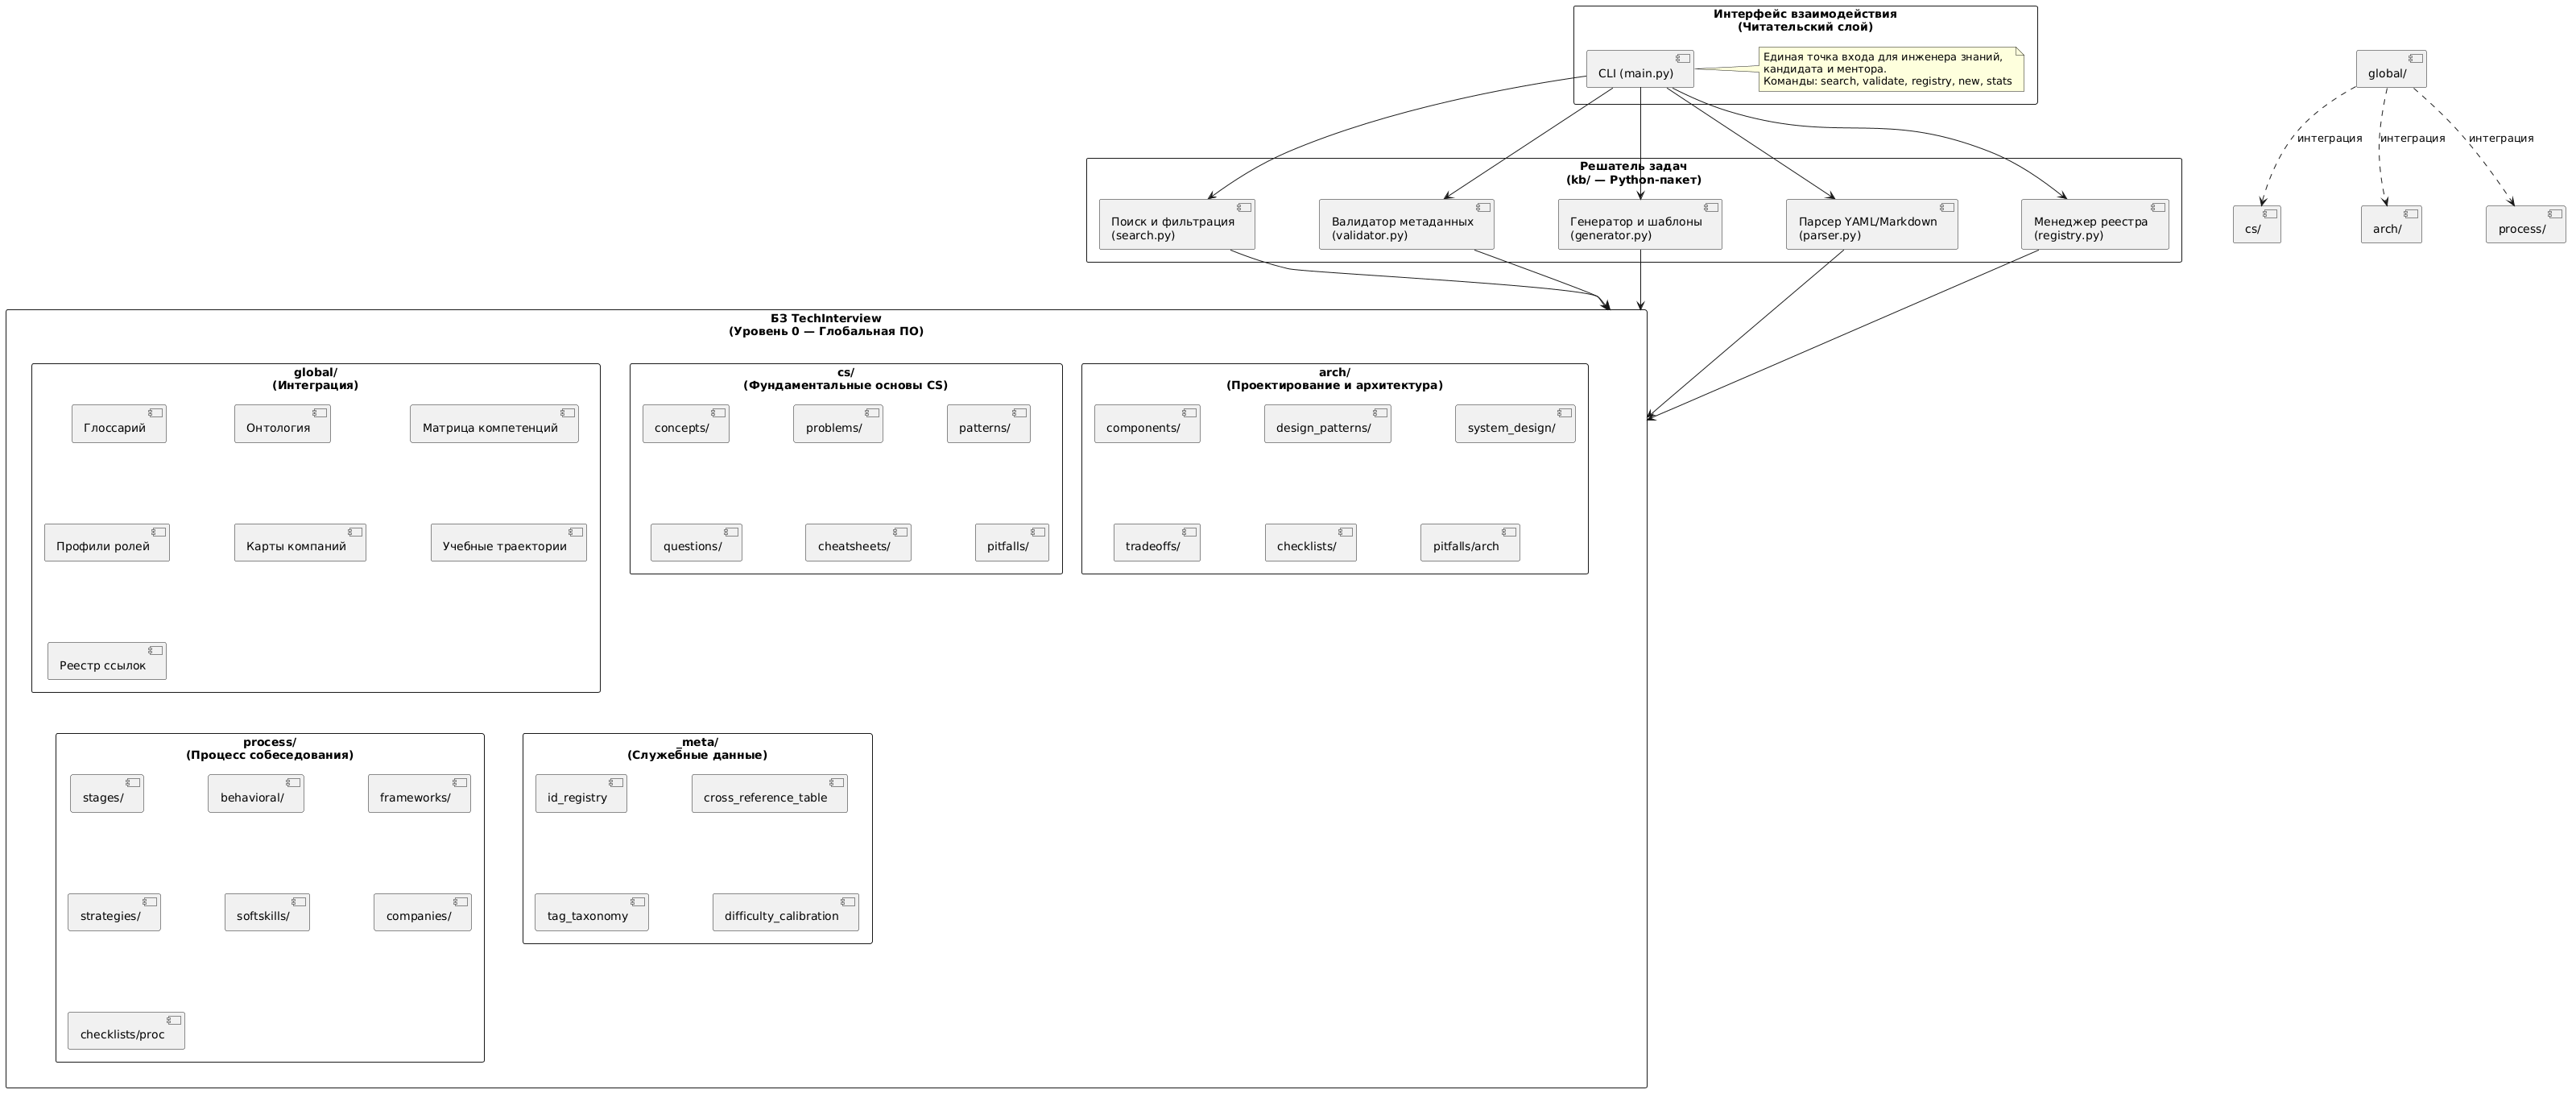
\includegraphics[width=1\textwidth]{picture/structure_of_the_knowledge_base.png}
    \caption{Уровневая организация базы знаний (Уровень 0 — глобальная ПО). Пунктирные линии обозначают интеграционные связи между глобальным слоем и доменными областями.}
    \label{fig:arch_level0}
\end{figure}

Согласно архитектурной схеме, представленной на рисунке \ref{fig:arch_level0}, система включает следующие функциональные компоненты:

\begin{itemize}
    \item \textbf{База знаний (Knowledge Base)} — файловое хранилище, структурированное по доменам (\texttt{cs/}, \texttt{arch/}, \texttt{process/}, \texttt{global/}) и категориям единиц знаний (\texttt{CONCEPT}, \texttt{PROBLEM}, \texttt{PATTERN}, \texttt{QUESTION}, \texttt{CHEATSHEET}, \texttt{PITFALL}).
    
    \item \textbf{Модуль логического вывода (Solver/Reasoner)} — слой на Python для семантического поиска, валидации метаданных, обработки графа зависимостей (\texttt{prerequisite\_for}), диагностики пробелов и построения адаптивных траекторий.
    
    \item \textbf{Слой взаимодействия (Interface Layer)} — CLI для инженеров знаний и веб-интерфейс (MVP) для пользователей. CLI покрывает создание, валидацию, поиск и отчёты, веб-слой — просмотр карточек, навигацию по связям и самопроверку.
    
    \item \textbf{Инфраструктурные сервисы} — Git для версионирования, внешние источники для верификации и автоматизированные тесты для контроля качества валидаторов и поисковых алгоритмов.
\end{itemize}

База знаний работает в \textbf{режиме чтения} для пользовательских сценариев; изменение данных выполняют только инженеры знаний через CLI с обязательной коммит-валидацией (формат метаданных, уникальность ID, целостность ссылок). Это обеспечивает воспроизводимость изменений и контроль качества.

Для предметной области CS дополнительно реализованы специализированные механизмы:
\begin{itemize}
    \item \textit{Калибровка сложности}: автоматическая привязка единиц знаний к уровням \texttt{junior}/\texttt{middle}/\texttt{senior} на основе метрик (асимптотическая сложность алгоритма, глубина требуемых пререквизитов, частота упоминания в собеседованиях).
    \item \textit{Граф алгоритмических зависимостей}: ориентированный ациклический граф, где вершины — концепции и задачи, а рёбра типа \texttt{prerequisite\_for} определяют допустимые последовательности изучения (например, \texttt{Массив} $\rightarrow$ \texttt{Двоичный поиск} $\rightarrow$ \texttt{Динамическое программирование}).
    \item \textit{Матрица компетенций}: таблица соответствия между единицами знаний и проверяемыми навыками (понимание асимптотического анализа, умение реализовывать обход графа, способность оптимизировать решение), используемая для диагностики и персонализации траекторий.
\end{itemize}

\subsection{Выбор формализма и логической основы}

\subsubsection*{Описание выбранного формализма}

% Требования:
% - указать выбранный формальный язык или структуру представления;
% - обосновать пригодность формализма для заявленных типов задач;
% - обосновать выразительную мощность и удобство последующей обработки.

Базовый формализм представления знаний — документно-ориентированный подход \textbf{Markdown + YAML-фронтматтер}. Выбор обусловлен следующими факторами:

\begin{enumerate}
    \item \textit{Соответствие предметной области:} Формат сочетает содержательный текст, код и диаграммы со строго типизированными метаданными, что необходимо для диагностики, планирования траекторий и генерации проверочных материалов.
    
    \item \textit{Выразительность и гибкость:} YAML поддерживает вложенные структуры и связи (\texttt{related}, \texttt{prerequisites}), а Markdown — код, таблицы и структурированный текст.
    
    \item \textit{Технологическая совместимость:} Формат обрабатывается стандартными библиотеками (\texttt{pyyaml}, \texttt{markdown}), совместим с Git и не требует специализированной СУБД.
    
    \item \textit{Эволюционная гибкость:} Новые метаданные добавляются без миграций и без нарушения работы существующих модулей.
    
    \item \textit{Машиночитаемость и человекочитаемость:} YAML обеспечивает формальную обработку, Markdown — удобство редактирования и рецензирования.
\end{enumerate}

На рисунке \ref{fig:unit_structure} представлена структура типовой единицы знаний на примере карточки концепции «Хеш-таблица», иллюстрирующая разделение метаданных (фронтматтер) и содержательной части, а также взаимосвязь атрибутов, ссылок на связанные документы и уровней детализации для разных уровней подготовки.

\begin{figure}[h]
    \centering
    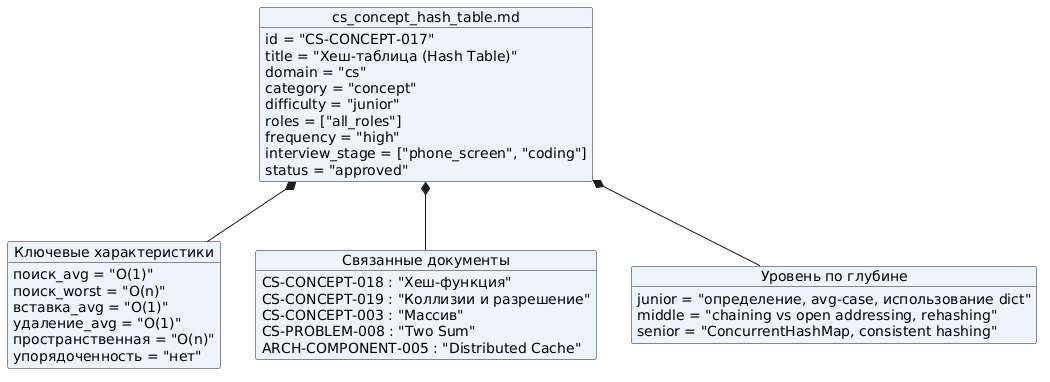
\includegraphics[width=0.85\textwidth]{picture/hash_table.png}
    \caption{Структура единицы знаний: взаимосвязь метаданных YAML, атрибутов, ссылок на связанные документы и уровней детализации.}
    \label{fig:unit_structure}
\end{figure}

\subsubsection*{Синтаксис и семантика}

% Требования:
% - указать основные синтаксические и семантические элементы формализма;
% - зафиксировать правила корректности;
% - не допускать смешение несовместимых формализмов.

Синтаксическая и семантическая организация БЗ определяется следующими правилами:

\begin{itemize}
    \item \textbf{Факты и сущности} задаются полями YAML-фронтматтера. Обязательный минимум (\texttt{id}, \texttt{title}, \texttt{domain}, \texttt{category}, \texttt{difficulty}) формирует контракт для автоматической обработки.
    
    \item \textbf{Отношения} фиксируются в \texttt{related} и \texttt{prerequisites}; используются типы связей \texttt{prerequisite\_for}, \texttt{depends\_on}, \texttt{evaluates}, \texttt{contrasts\_with}, \texttt{applied\_in}, \texttt{warns\_about}.
    
    \item \textbf{Ограничения целостности} включают проверку формата ID, допустимых значений перечислений, уникальности идентификаторов, валидности перекрёстных ссылок и наличия источников.
    
    \item \textbf{Правила генерации ID:} шаблон \texttt{[ДОМЕН]-[КАТЕГОРИЯ]-[НН]} (\texttt{CS-CONCEPT-017}, \texttt{CS-PROBLEM-008}) с трёхзначной нумерацией для сортируемости.
    
    \item \textbf{Таксономия тегов:} используются только теги из \texttt{\_meta/tag\_taxonomy.md}; произвольные значения запрещены.
\end{itemize}

Использование несовместимых формализмов не допускается; при интеграции с онтологическими системами предусмотрен экспорт YAML-метаданных в RDF/OWL.

\subsection{Концептуальная модель предметной области}

% Требования:
% - построить концептуальную модель предметной области: ключевые сущности, их свойства и отношения;
% - представить модель в виде диаграмм (UML-диаграммы классов);
% - пояснить, как структура концептов поддерживает решаемые задачи.

Концептуальная модель предметной области «Фундаментальные основы Computer Science» базируется на сущности \textbf{KnowledgeUnit}, от которой наследуются шесть категорий единиц знаний. Ключевые атрибуты: \texttt{id}, \texttt{title}, домен, категория, \texttt{difficulty}, \texttt{roles}, \texttt{tags}, \texttt{status}, \texttt{sources}, метаданные авторства и версионирования.

Отношения между сущностями формируют ориентированный ациклический граф знаний со следующими типами связей:
\begin{itemize}
    \item \textit{Иерархические и семантические:} \texttt{is\_part\_of}, \texttt{extends}, \texttt{relates\_to}, \texttt{contrasts\_with}, \texttt{alternative\_to}.
    \item \textit{Учебные и оценочные:} \texttt{prerequisite\_for}, \texttt{depends\_on}, \texttt{evaluates}, \texttt{applied\_in}, \texttt{warns\_about}.
\end{itemize}

\begin{figure}[h]
    \centering
    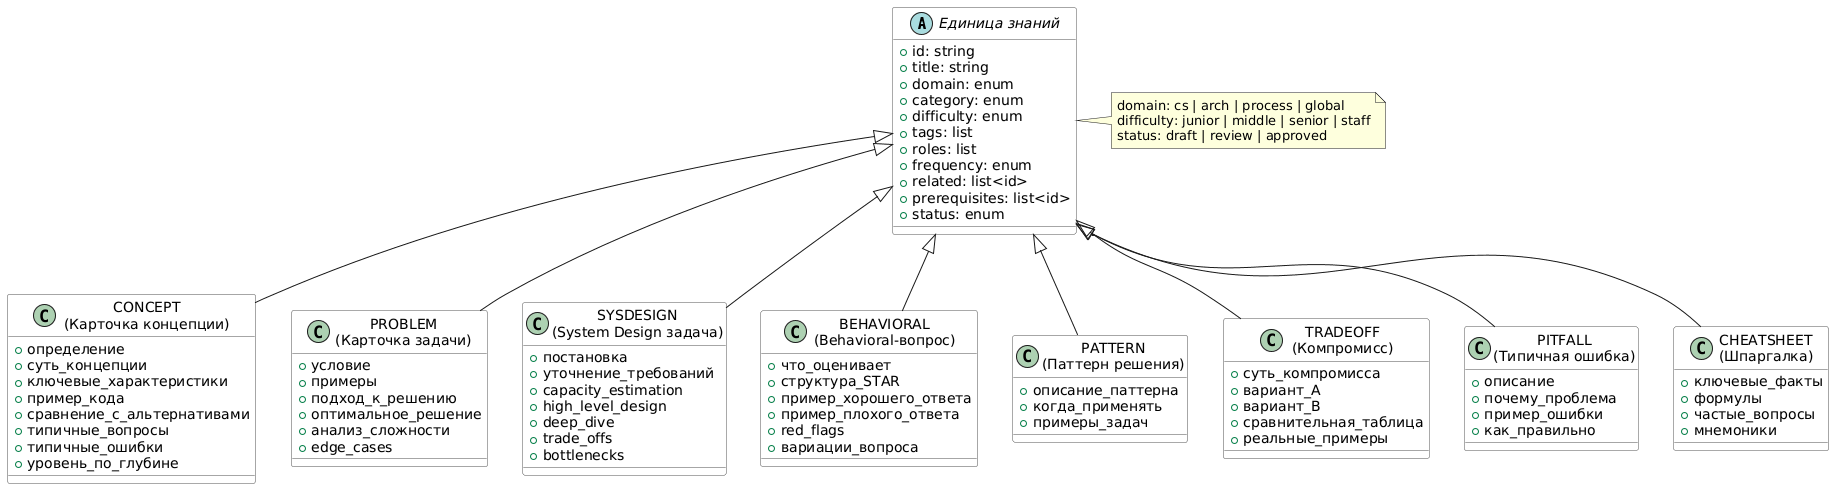
\includegraphics[width=0.95\textwidth]{picture/structure_of_subject_areas_and_types_of_knowledge_units.png}
    \caption{Концептуальная модель: иерархия классов единиц знаний и их специфические атрибуты для предметной области Computer Science.}
    \label{fig:conceptual_model}
\end{figure}

Структура концептов поддерживает ключевые задачи системы подготовки к собеседованиям:
\begin{itemize}
    \item Связи \texttt{prerequisite\_for} позволяют строить корректные последовательности изучения тем.
    \item Отношения \texttt{evaluates} поддерживают диагностику пробелов и персональные рекомендации.
    \item Единицы \texttt{PITFALL}/\texttt{CHEATSHEET}/\texttt{QUESTION}/\texttt{PROBLEM} обеспечивают самопроверку, предупреждения и повторение.
    \item Связи \texttt{applied\_in} и \texttt{exemplifies} показывают практическое применение теории в интервью-задачах.
\end{itemize}

Для предметной области CS дополнительно используются специализированные атрибуты: \texttt{time\_complexity\_*}, \texttt{space\_complexity} (алгоритмы), \texttt{input\_constraints}/\texttt{edge\_cases} (задачи), \texttt{pattern\_name}/\texttt{recognition\_hints} (паттерны), \texttt{common\_mistakes}/\texttt{how\_to\_avoid} (типичные ошибки).

\subsection{Логическая и физическая структура базы знаний}

\subsubsection*{Логическая структура}

% Требования:
% - описать иерархию классов, онтологические слои, модули;
% - указать, какие виды знаний хранятся в каждом модуле;
% - определить границы ответственности модулей.

Логическая организация БЗ реализована в иерархии каталогов, отражающей тематическую декомпозицию домена:

\begin{itemize}
    \item \textbf{\texttt{cs/concepts/} — Карточки концепций:} Теоретические материалы по структурам данных, алгоритмам и базовым принципам с примерами, сравнениями и уровнями детализации \texttt{junior}/\texttt{middle}/\texttt{senior}.
    
    \item \textbf{\texttt{cs/problems/} — Алгоритмические задачи:} Условия, примеры, ограничения, разборы решений, анализ сложности, edge cases и связи с концепциями/паттернами.
    
    \item \textbf{\texttt{cs/patterns/} — Паттерны решения задач:} Обобщённые стратегии (\texttt{Sliding Window}, \texttt{Two Pointers} и др.) с признаками распознавания, шаблонами и примерами.
    
    \item \textbf{\texttt{cs/questions/} — Вопросы собеседования:} Теоретические вопросы с эталонными ответами, критериями оценки и ссылками на релевантные концепции.
    
    \item \textbf{\texttt{cs/cheatsheets/} — Шпаргалки:} Краткие справочные материалы для быстрого повторения.
    
    \item \textbf{\texttt{cs/pitfalls/} — Типичные ошибки:} Распространённые ошибки кандидатов и рекомендации по их предотвращению.
\end{itemize}

Границы модулей задаются кодами домена и категории в идентификаторах. Модули изолированы по ответственности, но связаны единым пространством ID и кросс-доменными ссылками.

\subsubsection*{Физическая структура и форматы хранения}

% Требования:
% - описать физическое размещение базы знаний;
% - указать используемые форматы;
% - задать структуру каталогов/файлов.

Физически БЗ представляет собой файловое хранилище Markdown (\texttt{.md}, UTF-8). Каждая единица знаний хранится в отдельном файле с именем по шаблону \texttt{\{домен\}\_\{категория\}\_\{slug\}.md}.

Первичным ключом выступает поле \texttt{id} в YAML-фронтматтере. Для обеспечения нормализации применяется принцип единственного источника истины (SSOT): каждый факт описывается ровно один раз, повторное использование достигается через механизм перекрёстных ссылок. Файлы организованы в иерархическую структуру каталогов:

\begin{verbatim}
|-- concepts/   (data_structures/, algorithms/, ...)
|-- problems/   (arrays/, strings/, trees/, ...)
|-- patterns/
|-- questions/
|-- cheatsheets/
|-- pitfalls/
\end{verbatim}

Такая организация обеспечивает:
\begin{itemize}
    \item \textbf{Версионируемость и параллельную работу:} Git отслеживает изменения по файлам, что упрощает совместное редактирование.
    \item \textbf{Эффективный поиск:} Индексация метаданных позволяет фильтровать материалы без загрузки полного содержимого.
    \item \textbf{Масштабируемость и переносимость:} Добавление новых единиц не требует миграций, структура легко архивируется и переносится.
\end{itemize}

\subsection{Требования к программному прототипу (MVP)}
\label{sec:mvp}

\subsubsection*{Назначение и сценарии использования}

% Требования:
% - сформулировать цель создания прототипа;
% - показать сценарии использования через диаграмму прецедентов.

Программный прототип (MVP) — веб-интерфейс для демонстрации возможностей БЗ предметной области CS. Он выполняет роль читательского слоя, обеспечивая визуализацию связей, поиск и навигацию.

Основные сценарии использования отражены на диаграмме вариантов использования (Use Case) на рисунке \ref{fig:use_case}. Система поддерживает три роли пользователей, для каждой из которых определён набор доступных действий:

\begin{itemize}
    \item \textbf{Кандидат} — выполняет поиск и фильтрацию материалов, изучает карточки с адаптивной глубиной, проходит самопроверку и получает рекомендации.
    
    \item \textbf{Инженер знаний} — валидирует метаданные, управляет статусами (\texttt{draft}/\texttt{review}/\texttt{approved}), контролирует целостность ссылок и обновляет реестры.
    
    \item \textbf{Ментор / Технический интервьюер} — формирует вопросы и задачи под уровень кандидата, оценивает компетенции и строит планы подготовки.
\end{itemize}

\begin{figure}[h]
    \centering
    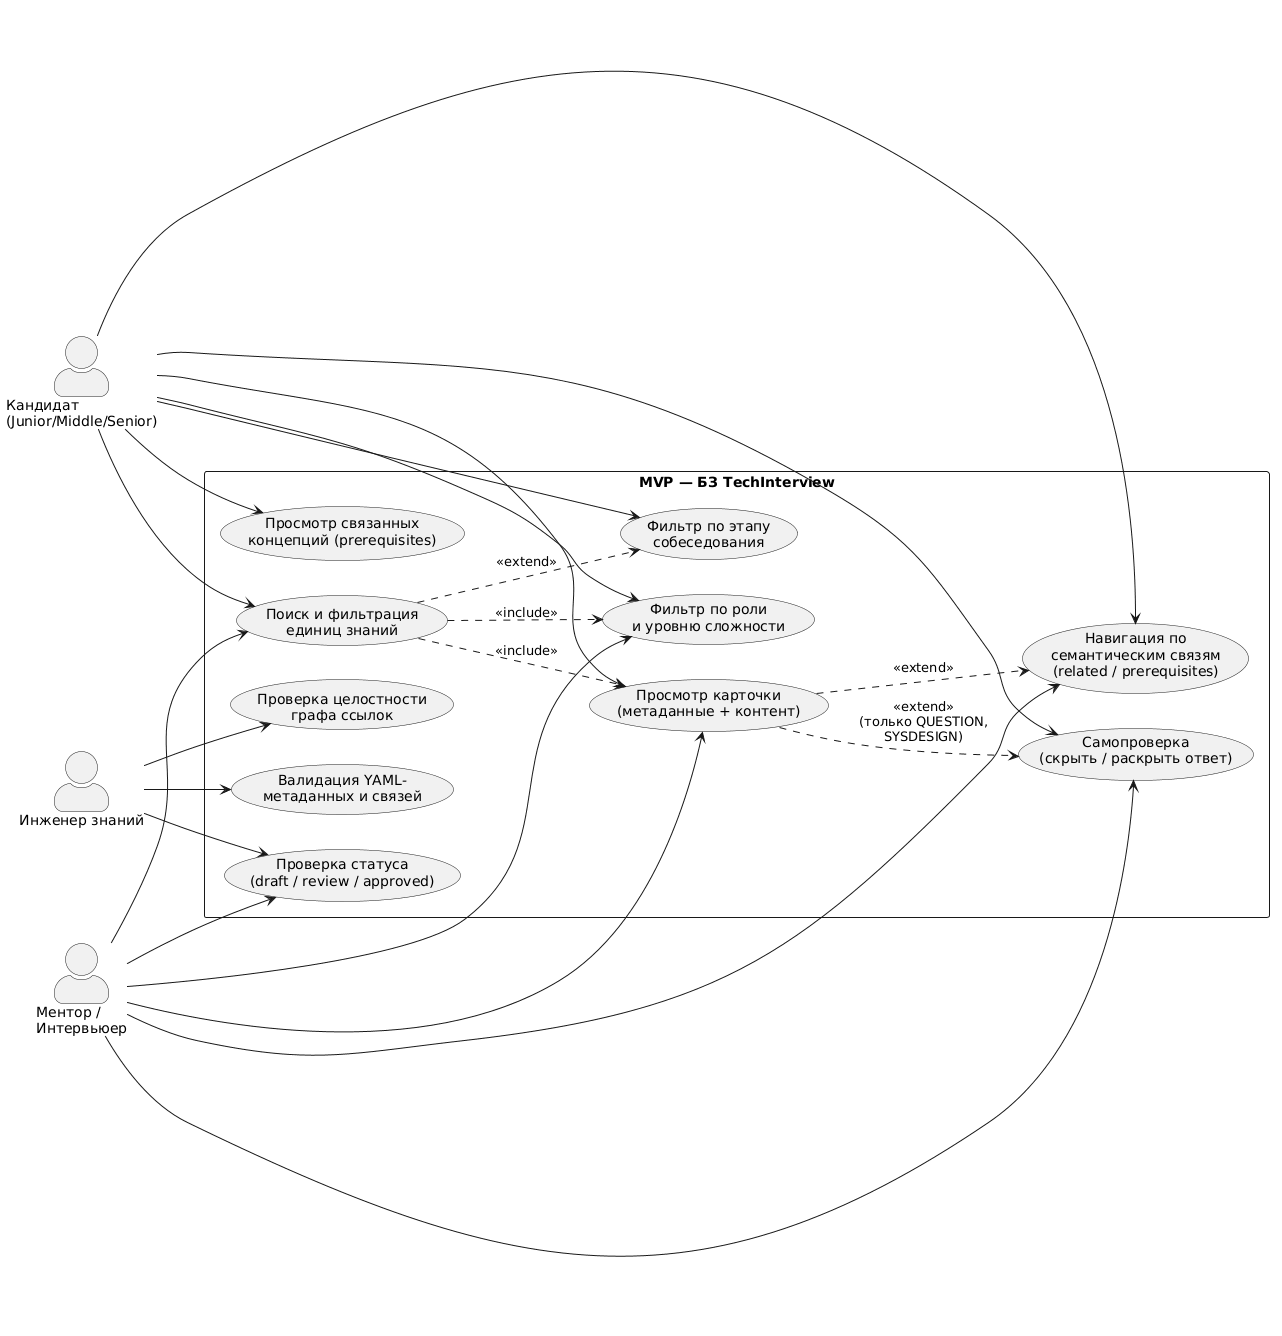
\includegraphics[width=0.9\textwidth]{picture/use_cases.png}
    \caption{Диаграмма вариантов использования (Use Case) MVP-приложения, отражающая роли и основные сценарии взаимодействия для предметной области CS.}
    \label{fig:use_case}
\end{figure}

\subsubsection*{Функциональные требования}

На основании сценариев использования к прототипу предъявляются следующие функциональные требования:

\begin{enumerate}
    \item Рендеринг единиц знаний с отображением YAML-метаданных и структурированного Markdown-контента.
    \item Комбинированный и полнотекстовый поиск по метаданным и содержимому с ранжированием релевантности.
    \item Интерактивная навигация по связям \texttt{related} и \texttt{prerequisites} с индикацией типа связи.
    \item Базовый режим самопроверки для \texttt{QUESTION}/\texttt{PROBLEM} со скрытием и последующим раскрытием эталонного ответа.
    \item Отображение статуса единицы знаний и адаптация глубины контента под уровни \texttt{junior}/\texttt{middle}/\texttt{senior}.
\end{enumerate}

\subsubsection*{Архитектурные решения}

Архитектура MVP реализована как одностраничное клиентское приложение (SPA) с локальным сервером статических файлов. Отказ от полноценного бэкенда обусловлен самодостаточностью \texttt{.md}-документов со встроенными метаданными.

\begin{figure}[h]
    \centering
    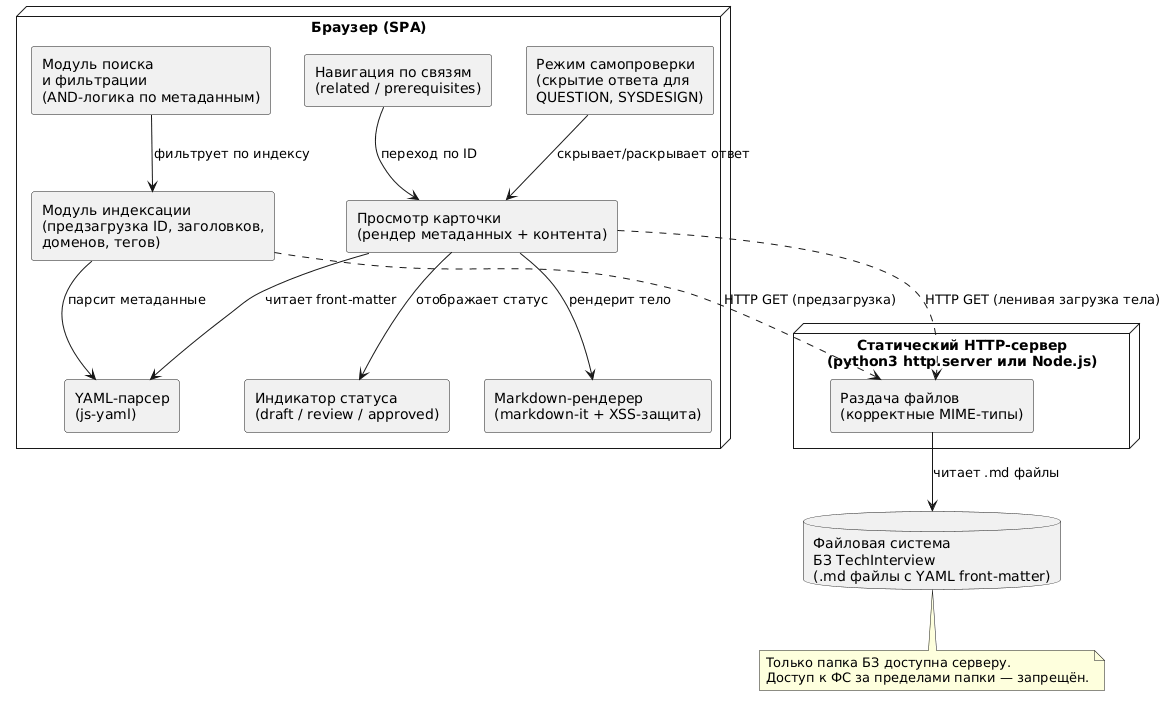
\includegraphics[width=0.95\textwidth]{picture/MVP_component_architecture.png}
    \caption{Архитектурная схема взаимодействия компонентов MVP: клиентская индексация метаданных, парсинг фронтматтера и ленивая загрузка содержимого документов.}
    \label{fig:mvp_arch}
\end{figure}

Как показано на рисунке \ref{fig:mvp_arch}, архитектура включает:
\begin{itemize}
    \item \textbf{Клиентский слой (Browser SPA):} 
    \begin{itemize}
        \item \textit{Модуль поиска и фильтрации:} работает с предзагруженным индексом метаданных (\texttt{\_meta/id\_registry.md}).
        \item \textit{YAML-парсер и Markdown-рендерер:} извлекают метаданные и отображают содержимое документа.
        \item \textit{Модуль навигации:} обрабатывает переходы по семантическим ссылкам и лениво загружает связанные документы.
    \end{itemize}
    
    \item \textbf{Серверный слой:} статический HTTP-сервер (например, \texttt{python3 -m http.server}) для раздачи файлов.
    
    \item \textbf{Файловая система:} Хранилище \texttt{.md} файлов, доступное в пределах корневой директории проекта, с иерархической структурой каталогов, отражающей логическую организацию знаний.
\end{itemize}

Такая архитектура обеспечивает быструю клиентскую фильтрацию, уменьшает сетевой трафик за счёт ленивой загрузки и упрощает развёртывание.

\subsection{Обеспечение согласованности, расширяемости и сопровождаемости}

% Требования:
% - описать механизмы контроля согласованности и непротиворечивости;
% - показать, как структура базы знаний позволяет добавлять новые факты без радикальной переработки;
% - выделить модули или уровни, отвечающие за разные аспекты предметной области.

\textbf{Механизмы контроля согласованности:}
\begin{enumerate}
    \item \textit{Типизация и перечисления:} YAML-фронтматтер валидируется по допустимым доменам, категориям, уровням сложности и статусам.
    \item \textit{ID и ссылки:} проверяются формат и уникальность идентификаторов, а также целостность \texttt{related}/\texttt{prerequisites}.
    \item \textit{Жизненный цикл и терминология:} статусы \texttt{draft}/\texttt{review}/\texttt{approved} и единый глоссарий предотвращают попадание несогласованных материалов в рабочий контур.
\end{enumerate}

\textbf{Расширяемость и модульность:}
\begin{enumerate}
    \item \textit{Доменная изоляция:} независимое развитие доменов без взаимного влияния.
    \item \textit{Документно-ориентированное хранение:} добавление новой единицы сводится к созданию одного файла без миграций.
    \item \textit{Динамический реестр и расширяемая схема:} автоматическая генерация \texttt{\_meta/id\_registry.md} и добавление новых YAML-полей без нарушения совместимости.
\end{enumerate}

\textbf{Сопровождаемость и документирование:}
\begin{enumerate}
    \item \textit{Шаблоны и CLI-инструменты:} стандартизируют структуру единиц знаний и автоматизируют операции (\texttt{new}, \texttt{validate}, \texttt{registry}, \texttt{stats}, \texttt{search}).
    \item \textit{Тестирование:} набор из 177 тестов (\texttt{pytest}) покрывает парсинг, валидацию, поиск и генерацию.
    \item \textit{Документация:} \texttt{CONTRIBUTING.md} и \texttt{TERMINAL\_GUIDE.md} задают правила добавления и сопровождения контента.
\end{enumerate}

\subsection{Вывод по разделу проектирования}

% Требования:
% - кратко зафиксировать ключевые проектные решения;
% - указать, как они обеспечивают выполнение требований;
% - отметить предусмотренные возможности расширения и контроля качества.

В ходе проектирования базы знаний \texttt{TechInterview} для предметной области «Фундаментальные основы Computer Science» приняты следующие ключевые решения:

\begin{enumerate}
    \item \textbf{Формализм Markdown + YAML:} обеспечивает баланс человекочитаемости и машиночитаемости, поддерживает декларативные и процедурные знания и допускает эволюцию схемы метаданных.
    \item \textbf{Многоуровневая модульная архитектура:} декомпозиция по доменам и интеграционный слой обеспечивают кросс-доменные связи без дублирования и упрощают сопровождение.
    \item \textbf{Инструментальная поддержка качества:} CLI-валидация, реестр связей и автоматизированные тесты (177 случаев) снижают число ошибок и стабилизируют развитие БЗ.
    \item \textbf{Подготовка к адаптивному решателю:} унифицированные ID, граф семантических связей и матрица компетенций обеспечивают основу для диагностики пробелов, персональных рекомендаций и масштабирования.
\end{enumerate}

Принятые решения соответствуют назначению системы: формируют надёжный, расширяемый и семантически связный источник знаний для подготовки к техническим собеседованиям. Архитектура сохраняет баланс между строгостью автоматизированной обработки и практической удобностью для авторов и пользователей, создавая основу для дальнейшей интеграции адаптивных модулей и расширения предметного покрытия.